\documentclass{standalone}
\usepackage{tikz}
\usepackage{pgfplots}
\pgfplotsset{width=32cm,height=18cm,compat=1.3}
\pgfplotsset{every tick label/.append style={font=\Huge}}
\usepackage{filecontents}

\usetikzlibrary{patterns}

\definecolor{citrine}{rgb}{0.89, 0.82, 0.04}
\definecolor{arylideyellow}{rgb}{0.91, 0.84, 0.42}
\definecolor{bronze}{rgb}{0.8, 0.5, 0.2}

\begin{document}
	\centering
		\vspace{1.5em}
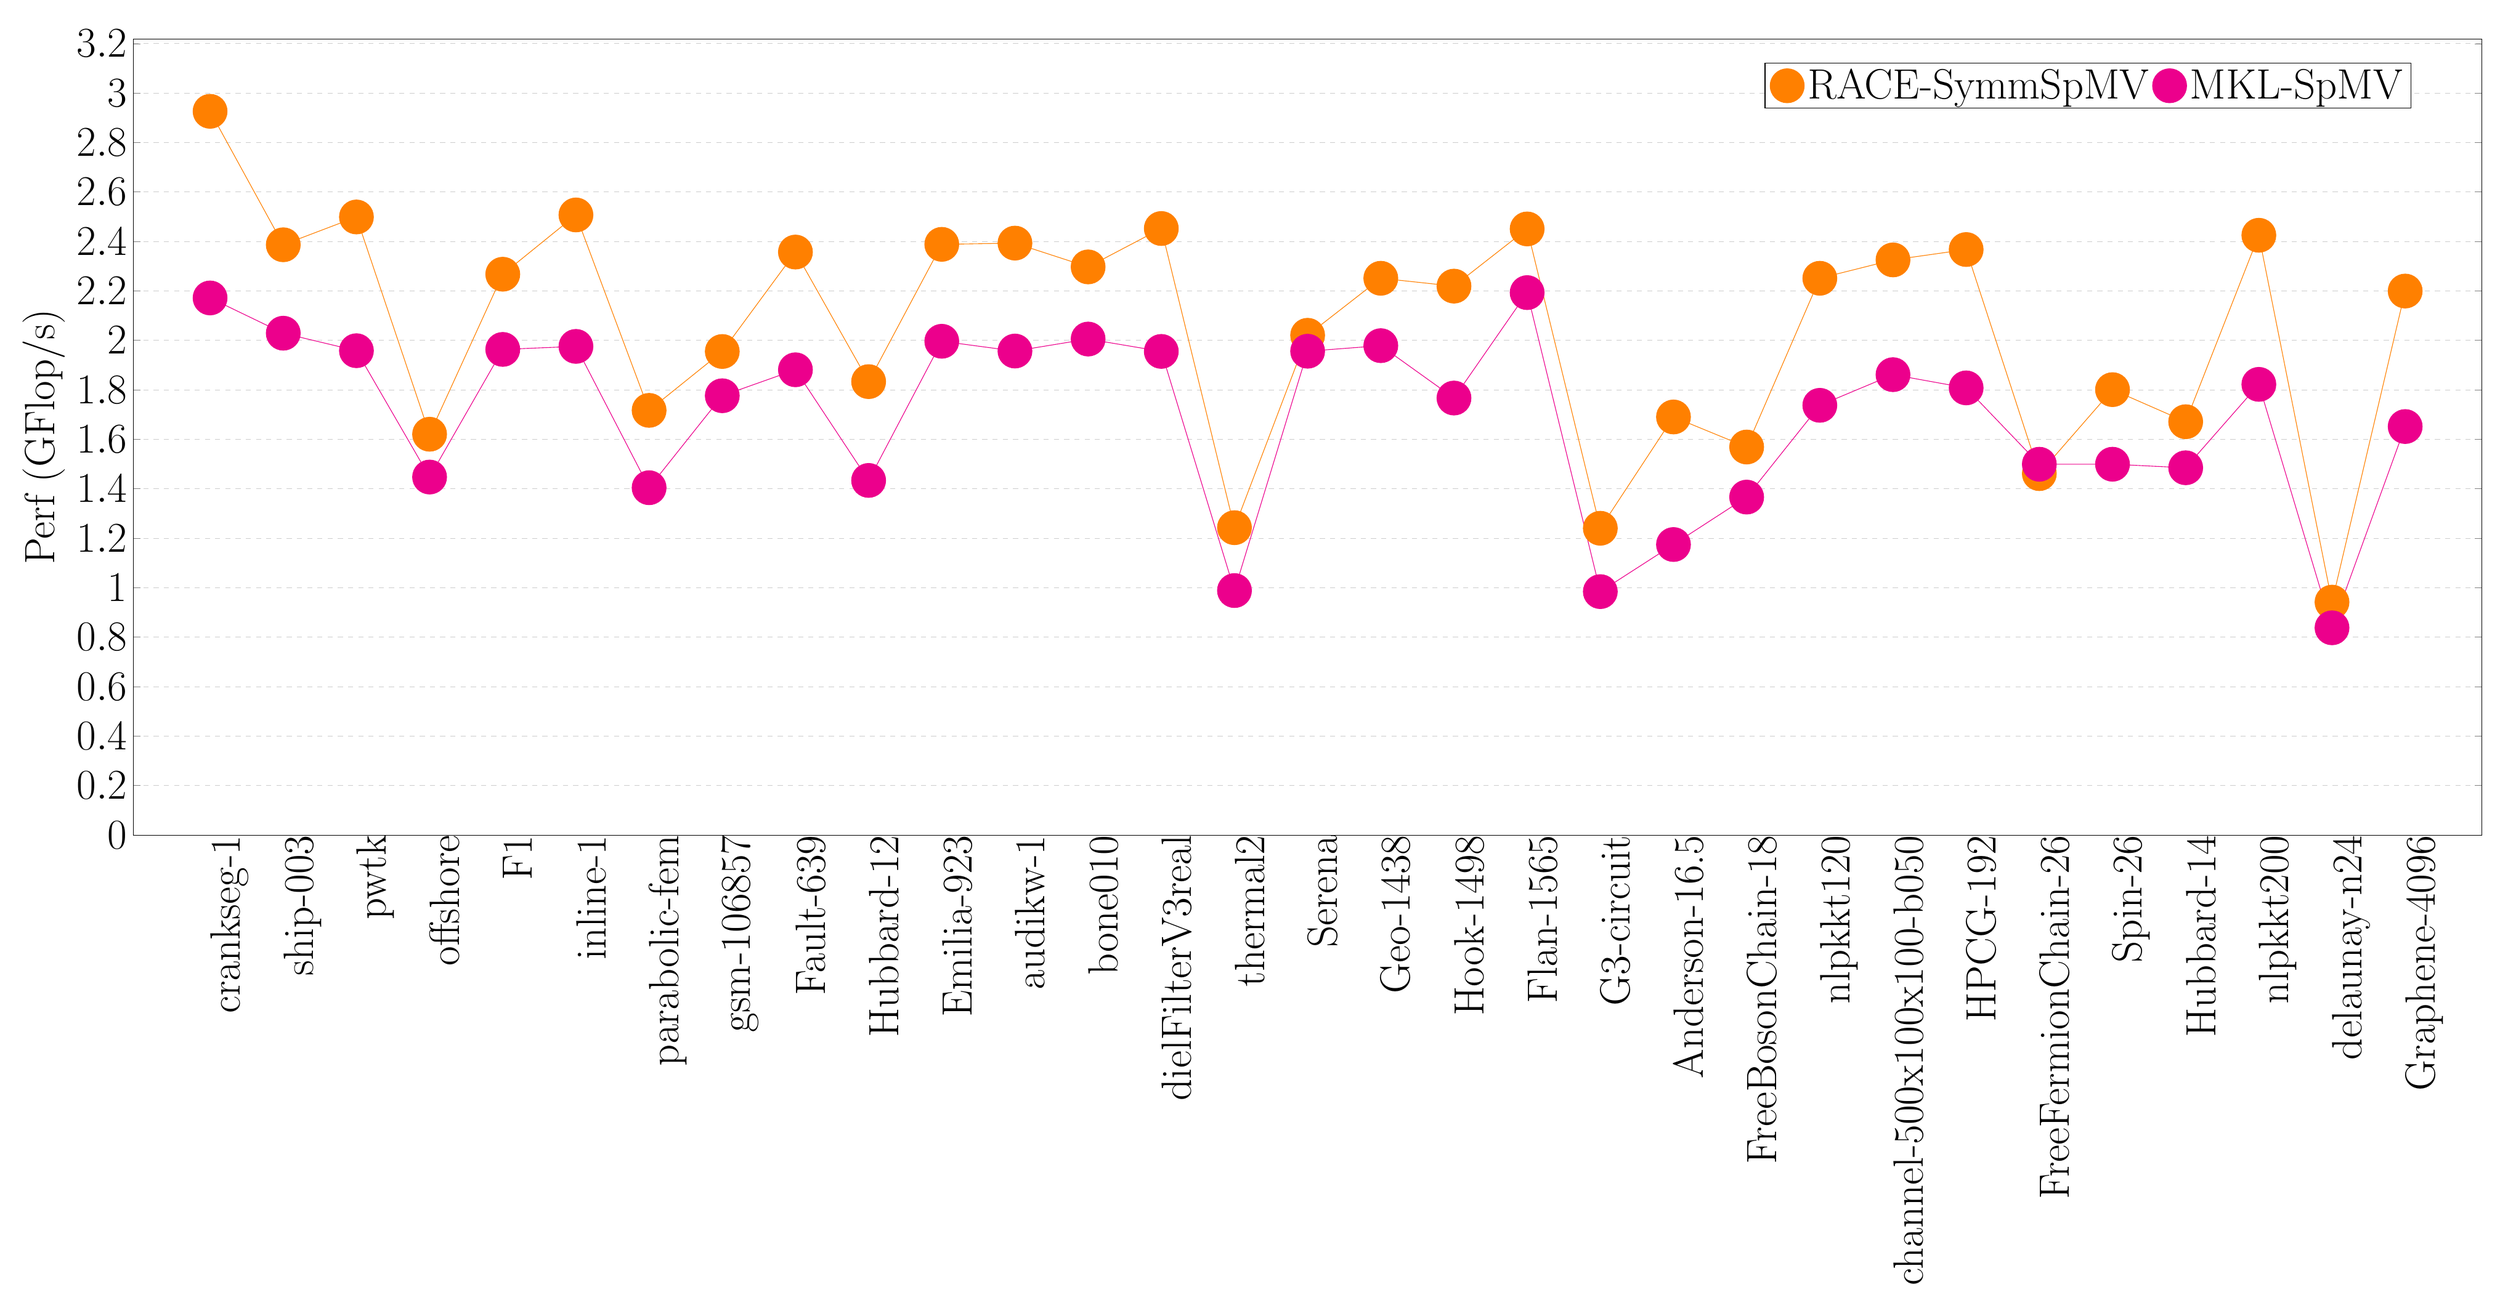
\begin{tikzpicture}
		%	\node at (13.25,15) {\LARGE{}};
			\begin{axis}[
		%	xmin=0.25, xmax=7.25,
			ymin=0, %ymax=3.25,
			xtick={1, 2, 3, 4, 5, 6, 7, 8, 9, 10, 11, 12, 13, 14, 15, 16, 17, 18, 19, 20, 21, 22, 23, 24, 25, 26, 27, 28, 29, 30, 31},
		%	ytick={0,0.5,1,1.5,2,2.5,3},
			xticklabels={crankseg-1, ship-003, pwtk, offshore, F1, inline-1, parabolic-fem, gsm-106857, Fault-639, Hubbard-12, Emilia-923, audikw-1, bone010, dielFilterV3real, thermal2, Serena, Geo-1438, Hook-1498, Flan-1565, G3-circuit, Anderson-16.5, FreeBosonChain-18, nlpkkt120, channel-500x100x100-b050, HPCG-192, FreeFermionChain-26, Spin-26, Hubbard-14, nlpkkt200, delaunay-n24, Graphene-4096},
			width  = 50cm,
			height = 18cm,
			major x tick style = transparent,
			%	minor ytick={1, 5, 10, 15, 20, 25, 30 ,35,40},
			grid = minor,	
			%add_bar_commands
			ymajorgrids = true,
			grid style={dashed, gray!40},
			ylabel = {\Huge{Perf (GFlop/s)}},
		%	symbolic x coords={Graphene-2048-2048, Graphene-4096-4096, Spin-24-24-24},
			x tick label style={rotate=90, anchor=north east, inner sep=0mm, font={\Huge}},
			tick label style={font={\Huge}},
			scaled y ticks = false,
			enlarge x limits=0.035,
			legend cell align=left,
			legend style={font=\Huge},
			legend columns=-1,
			legend style={
				%at={(1,1.05)},
				%anchor=south east,
				%column sep=1ex,
				legend pos=north east
			},
			%spl_legend_code
			title= {\Huge\scalebox{1.5}{{}}}
			]

\addplot[ mark=*, mark size=10pt, mark options={orange}, draw=orange ] plot coordinates{(1,2.926099) (2,2.386563) (3,2.499016) (4,1.620525) (5,2.267526) (6,2.507186) (7,1.717044) (8,1.955117) (9,2.357104) (10,1.833257) (11,2.388295) (12,2.393282) (13,2.297065) (14,2.452344) (15,1.242718) (16,2.020670) (17,2.251098) (18,2.219353) (19,2.450631) (20,1.240375) (21,1.690370) (22,1.568837) (23,2.251105) (24,2.325366) (25,2.367308) (26,1.461291) (27,1.800820) (28,1.671180) (29,2.424999) (30,0.941774) (31,2.199443)};
\addplot[ mark=*, mark size=10pt, mark options={magenta}, draw=magenta ] plot coordinates{(1,2.171627) (2,2.029020) (3,1.958276) (4,1.447446) (5,1.963496) (6,1.975699) (7,1.404327) (8,1.776152) (9,1.881138) (10,1.433767) (11,1.996419) (12,1.956905) (13,2.005389) (14,1.955419) (15,0.988494) (16,1.956167) (17,1.978657) (18,1.766859) (19,2.193155) (20,0.984235) (21,1.174614) (22,1.366403) (23,1.737451) (24,1.861416) (25,1.807951) (26,1.499220) (27,1.499291) (28,1.484987) (29,1.822177) (30,0.837903) (31,1.651648)};
	%addplot cmd

	\legend{RACE-SymmSpMV, MKL-SpMV}

	\end{axis}			
\end{tikzpicture}

\end{document}

